\documentclass{article}

% if you need to pass options to natbib, use, e.g.:
%     \PassOptionsToPackage{numbers, compress}{natbib}
% before loading neurips_2020

% ready for submission
% \usepackage{neurips_2020}

% to compile a preprint version, e.g., for submission to arXiv, add add the
% [preprint] option:
    % \usepackage[preprint]{neurips_2020}

% to compile a camera-ready version, add the [final] option, e.g.:
%     \usepackage[final]{neurips_2020}

% to avoid loading the natbib package, add option nonatbib:
\usepackage[nonatbib,preprint]{neurips_2020}

\usepackage[utf8]{inputenc} % allow utf-8 input
\usepackage[T1]{fontenc}    % use 8-bit T1 fonts
\usepackage{hyperref}       % hyperlinks
\usepackage{url}            % simple URL typesetting
\usepackage{booktabs}       % professional-quality tables
\usepackage{amsfonts}       % blackboard math symbols
\usepackage{nicefrac}       % compact symbols for 1/2, etc.
\usepackage{microtype}      % microtypography
\usepackage{graphicx}
\title{How Do We Calculate the Livability of Manhattan's Neighborhoods?}
\begin{document}
\maketitle
\section{Background}
People seeking to find the ideal place to live in Manhattan often face challenges in obtaining helpful information. Existing resources like the AARP$^{[2]}$ Livability Index offer some guidance, but they may not be tailored to a specific demographic. This project aims to address this by identifying and measuring the livability of Manhattan neighborhoods for different age groups. We will investigate factors like transportation access, housing affordability, and restaurant density to understand how they affect a neighborhood's overall livability. The project's value lies in assisting individuals to improve their quality of life and aiding governments in making informed decisions about resource allocation and policy design.

To achieve our goal, we utilized various datasets, as mentioned in the following section, to extract information about businesses, services, restaurants, grocery shops, apartment rents, and sentiments of population based on location. We utilized publicly available data and fetched information of businesses, other services, and trends in each neighborhood using public third-party APIs. 

\section{Datasets}
We are using data from many sources in order to determine different elements of the livability score for each neighborhood, as shown below: 
\begin{enumerate}
  \item We are using Yelp's Fusion Open API to get restaurants and business data from Yelp across more than 100 categories. We are curating our dataset from the response data of Fusion API for about 1100+ businesses (restaurants, services) across Manhattan. Total size of business and categories datasets is 100 MB.
  \item We are using a 26 KB dataset from NYC Open Data that contains latitude and longitude values for the center of each neighborhood in Manhattan in order to classify each data point from our other datasets into a neighborhood.
  \item We are using a dataset from Streeteasy that contains the median rental prices in each neighborhood for different sizes of apartments (studio up to three bedroom apartments).  This dataset is 1.3 MB in size and its features include monthly median rental prices for each month in each neighborhood for the past ~10 years.
  \item We are also using a 468 KB dataset that contains the latitude and longitude coordinates of subway stations in Manhattan.
  \item We are using Twitter$^{[3]}$ data, where we extracted the tweet content posted between 14th April and 28th April for each neighborhood. After thorough filtering and cleaning, the expected data size is around 80 MB. 
  \item Doordash Restaurants and Recognized Grocery Stores datasets were also used for further analysis. The Doordash Restaurant dataset obtained from Kaggle is 4.8 MB, while the Recognized Grocery Stores dataset obtained from NYC OpenData is 49 KB. 
\end{enumerate}

\section{Analysis}
We curated most of our datasets either from other available datasets or from public APIs from Yelp and Twitter by extracting the most relevant information affecting the livability of a neighbourhood. We found that most of the data based on location includes latitude and longitude information and felt the need to curate a common mapping logic to map each data to a neighbourhood. We identified the centroid lat,long for each neighbourhood and created neighbourhood name column for each dataset using this mapping logic, to join our results based on neighbourhood names. 

Some of the data cleaning steps we have taken include removing all the rows of data from boroughs outside of Manhattan and backward filling missing values (in the case of the Streeteasy dataset). For twitter, we need to process data by conducting language filtering, removing @mentions, discarding tweets containing only URLs, excluding tweets not relevant to the neighborhood, and determining the location of each tweet. For Yelp dataset, we removed invalid data rows, and included only the most important data based on review counts and average ratings to disregard outliers. For Doordash Restaurants and Grocery Stores datasets, we defined a new dataframe with only the relevant data, including the restaurant/grocery store information and geographic location. 

One issue we faced is defining the boundaries of each neighborhood.  We found datasets that contain many latitude and longitude coordinates outlining each neighborhood’s boundary, but we decided that using such dataset would pose more challenges to calculating the neighborhood of a single coordinate point as opposed to comparing that coordinate to the closest neighborhood centroid.

On Twitter data, our analysis involves the utilization of NLP via TextBlob's$^{4}$ Naive Bayes classifier to perform sentiment analysis. Through this classification, we are able to measure both the polarity and subjectivity of the content within each tweet.

We used data from MTA to calculate the number of subway station entrances in each neighborhood.  Since each subway station entrance was not assigned to a neighborhood in the MTA dataset, we determined each data point's neighborhood using our custom function that calculates the distance between the latitude and longitude values of the data point with that of the neighborhood centroids to find the most likely neighborhood for each data point.

In order to assign weights to each dataset according to the age, we rely on research$^{[6]}$ to determine the significance of each factor for different age groups. These findings are then applied to calculate the ultimate scores for each neighborhood as shown below.\\
for a user age $j$, we derive weight of each category:
\newpage
$w_q$: Weight of neighborhood quality

$w_c$: Weight of convenience to public transport

$w_a$: Weight of affordability from the prior study

For a neighborhood $i$, we can then derive the following scores:

$score_{twitter}$: Score associated with Twitter activity

$score_{doordash}$: Score associated with DoorDash activity

$score_{grocery}$: Score associated with grocery availability

$score_{mta}$: Score associated with MTA (Metropolitan Transportation Authority) convenience

$score_{streeteasy}$: Score associated with StreetEasy (real estate marketplace) activity\\
The final score can be calculated using the following formula:\\

\begin{figure}[h]
\centering
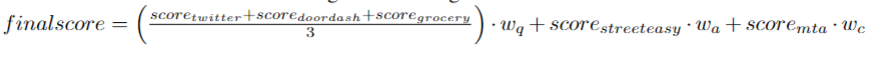
\includegraphics[scale=0.6]{picpuic.png}
\end{figure}


\section{Results}
One aspect of the results includes the number of positive/negative sentiment tweets and the average sentiment score for each neighborhood. The sentiment score scale ranges from -1 to 1, with a score of 1 denoting a highly positive sentiment and a score of -1 indicating a neutral sentiment. Our underlying hypothesis is that if someone is in a neighborhood, for example, “Roosevelt Island”, and tweets something positive that has the word “Roosevelt Island”, then it implies higher livability for “Roosevelt Island”. The capture below shows the sentiment score of each neighborhood and the proportion of positive tweets of the top 10 neighborhoods that have the highest number of tweets.

\begin{figure}[h]
\centering
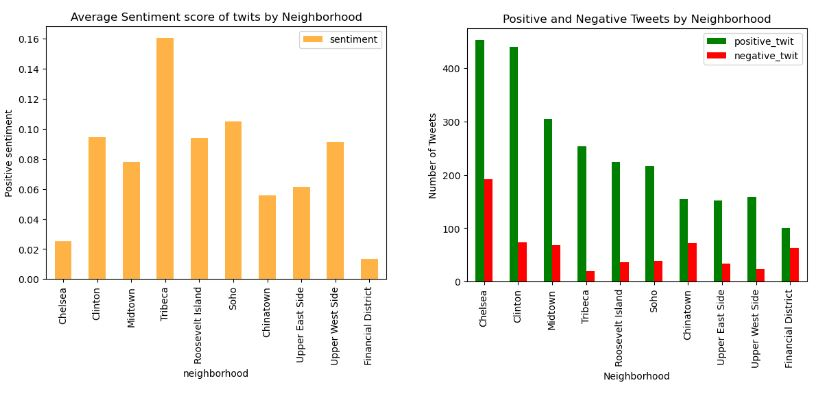
\includegraphics[scale=0.50]{init_twitter.JPG}
\end{figure}

We also used the Streeteasy dataset to determine a “trendiness”, where we used to calculate the recent levels of demand for neighborhoods.  Below, we plot the neighborhoods we consider to be the most “trendy”, where prices have risen the most in the past few years. Chelsea, Flatiron, and West Village appear to be the most trendy neighborhoods, which confirms our prior suspicions.  We believe that if prices are rapidly increasing for a neighborhood, it serves as an indication of higher livability since there is higher demand in that neighborhood than elsewhere.

\begin{figure}[h]
\centering
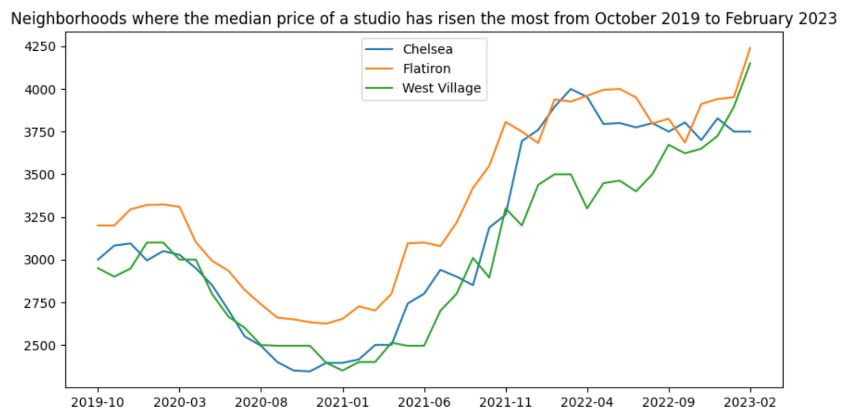
\includegraphics[scale=0.50]{init_median.JPG}
\end{figure}

Another factor of livability regarding apartment prices is affordability.  We took the median price for all apartment types (studio, one bedroom, two bedroom, three+ bedroom, and coop) for each neighborhood and calculated the average price over the last thirteen years.  From those values, we normalized them from a score of 0 to 100. Once we had those scores, where a higher score indicated a higher rent price, we subtracted 100 from each of those values to invert the scores.  So now, the neighborhoods with lower rent prices (more affordable) have a higher score than neighborhoods with higher rent prices.  We then used these "affordability" scores to calculate the final "livability" score in the end.

\begin{figure}[h]
\centering
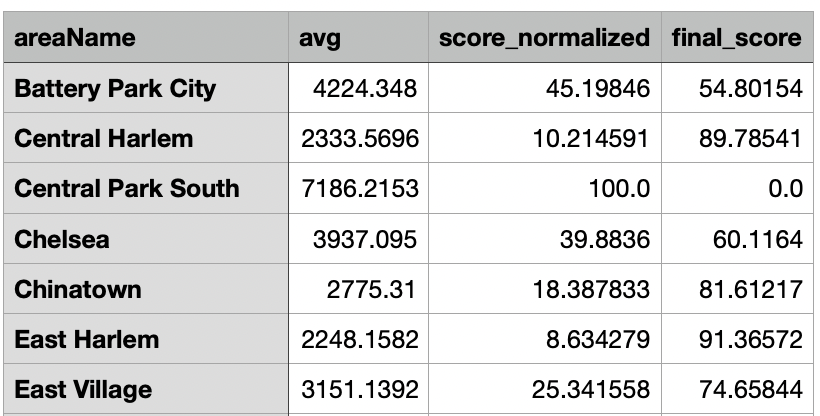
\includegraphics[scale=0.50]{streeteasy.JPG}
\end{figure}

From Yelp, Doordash and Grocery Stores datasets, we computed the total number of restaurants, grocery stores and businesses within each neighborhood along with their types and user ratings. The results helped us determine the quality of life provided by the neighborhood based on the available options of delivery, shopping, services and grocery stores and in terms of proximity for its residents. As shown below, for the Doordash Restaurants as well as the Grocery Stores datasets, we calculated the total number of restaurants and grocery stores in the neighborhoods presented in the datasets. From the count of restaurants and grocery stores, we normalized the values from a score of 0 to 1; a neighborhood with a normalized score of 1 indicated that it has the most number of services, and so provides the best quality of life for its residents. 

\begin{figure}[h]
\centering
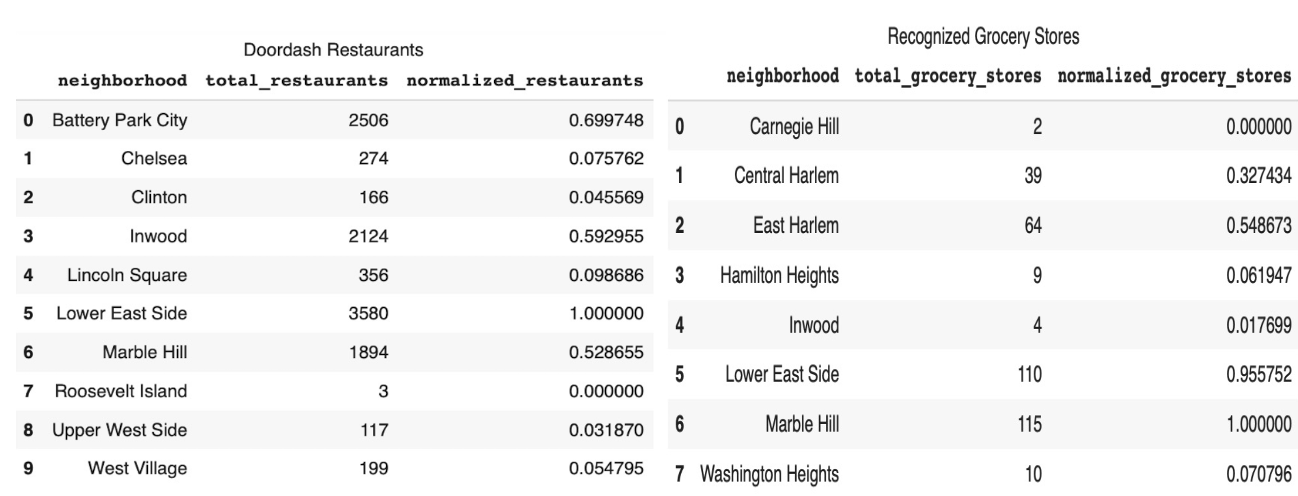
\includegraphics[scale=0.5]{Normalized.png}
\end{figure}

\begin{figure}[h]
\centering
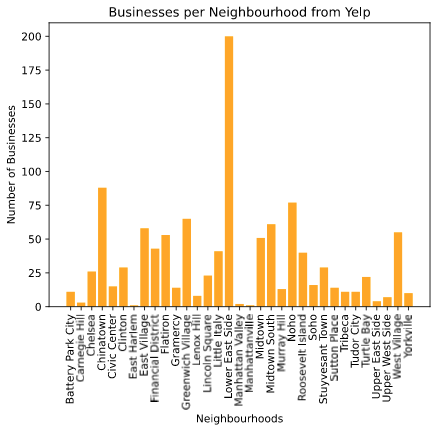
\includegraphics[scale=0.5]{from_yelp.png}
\end{figure}

\newpage

Another important consideration of livability is convenience.  We define convenience of a neighborhood as having a high number of subway stations.  We analyzed a dataset containing all the MTA subway stations in New York City and calculated how many subway entrances are in each neighborhood.  We then normalized the number of subway entrances between 0 and 100 to be used in our final calculation of livability, with a higher score indicating more subway entrances and thus higher convenience for a neighborhood. 

\begin{figure}[h]
\centering
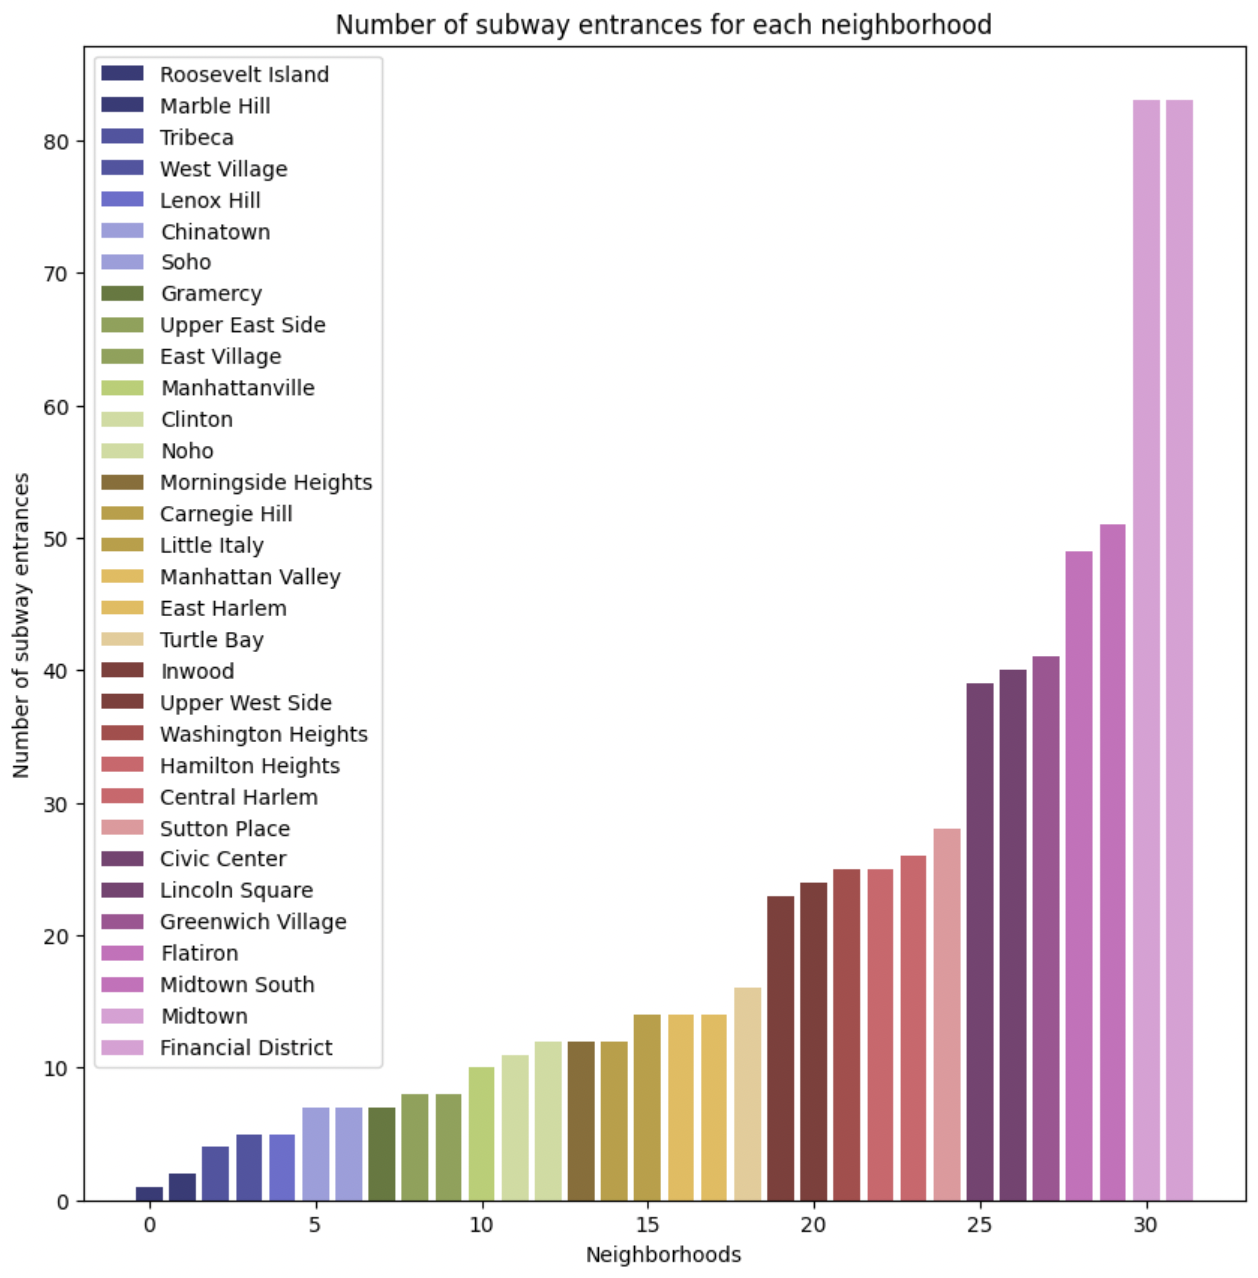
\includegraphics[scale=0.50]{mta.JPG}
\end{figure}

Here are the final results and the scores broken down for each category.  

We used weights for three different categories to determine the final output for each neighborhood: quality of neighborhood (as given by Twitter sentiment data, DoorDash data, and grocery store data), affordability (as given by Streeteasy rental price data), and convenience (as given by the MTA subway station data).  We determined the weights based on research$^{[5]}$ that reflected the importance of each one of these categories to different age groups of residents. We used those weights to calculate the final livability scores for each neighborhood in our study. 

\begin{figure}[h]
\centering
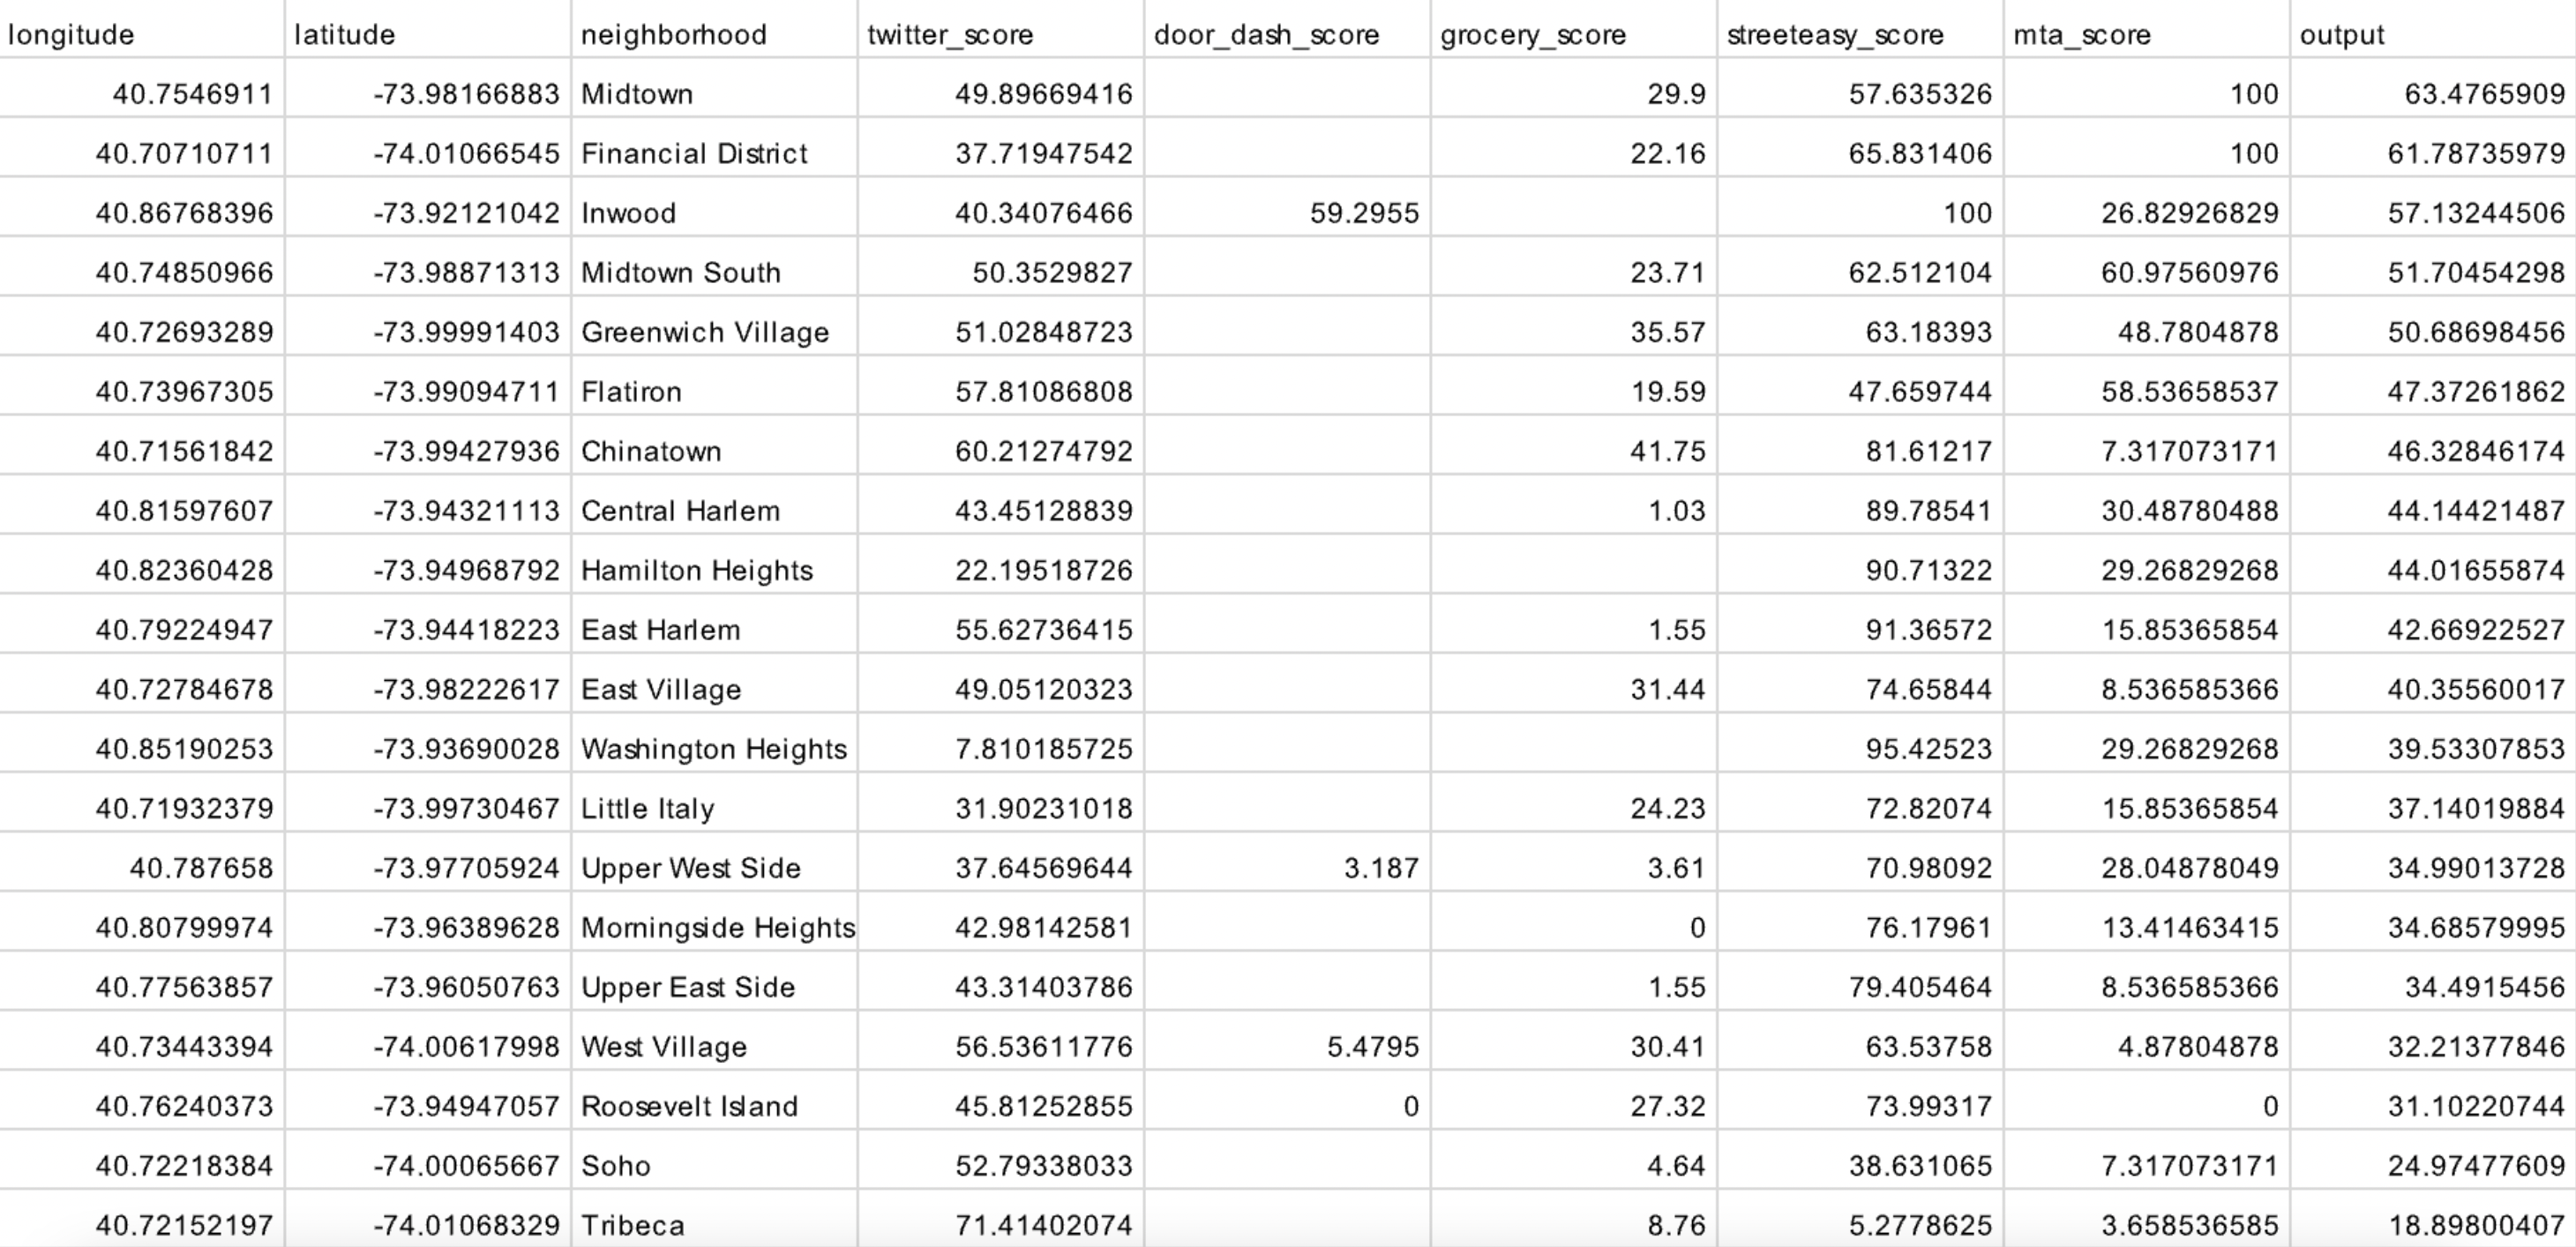
\includegraphics[scale=0.30]{final_results_broken_down.JPG}
\end{figure}

Below are the final rankings for each neighborhood by age groups.  Midtown, Financial District, and Inwood placed in the top 3 for most age demographics.  We found that these three neighborhoods are most popular for the younger age groups.  We believe this is due to the fact that younger people optimize for convenience to public transportation and access to restaurants and grocery stores when choosing a neighborhood.  On the other hand, we noticed that older age groups prefer neighborhoods that are quieter and more affordable since many older folks are living on their retirement savings.
\newpage
\begin{figure}[h]
\centering
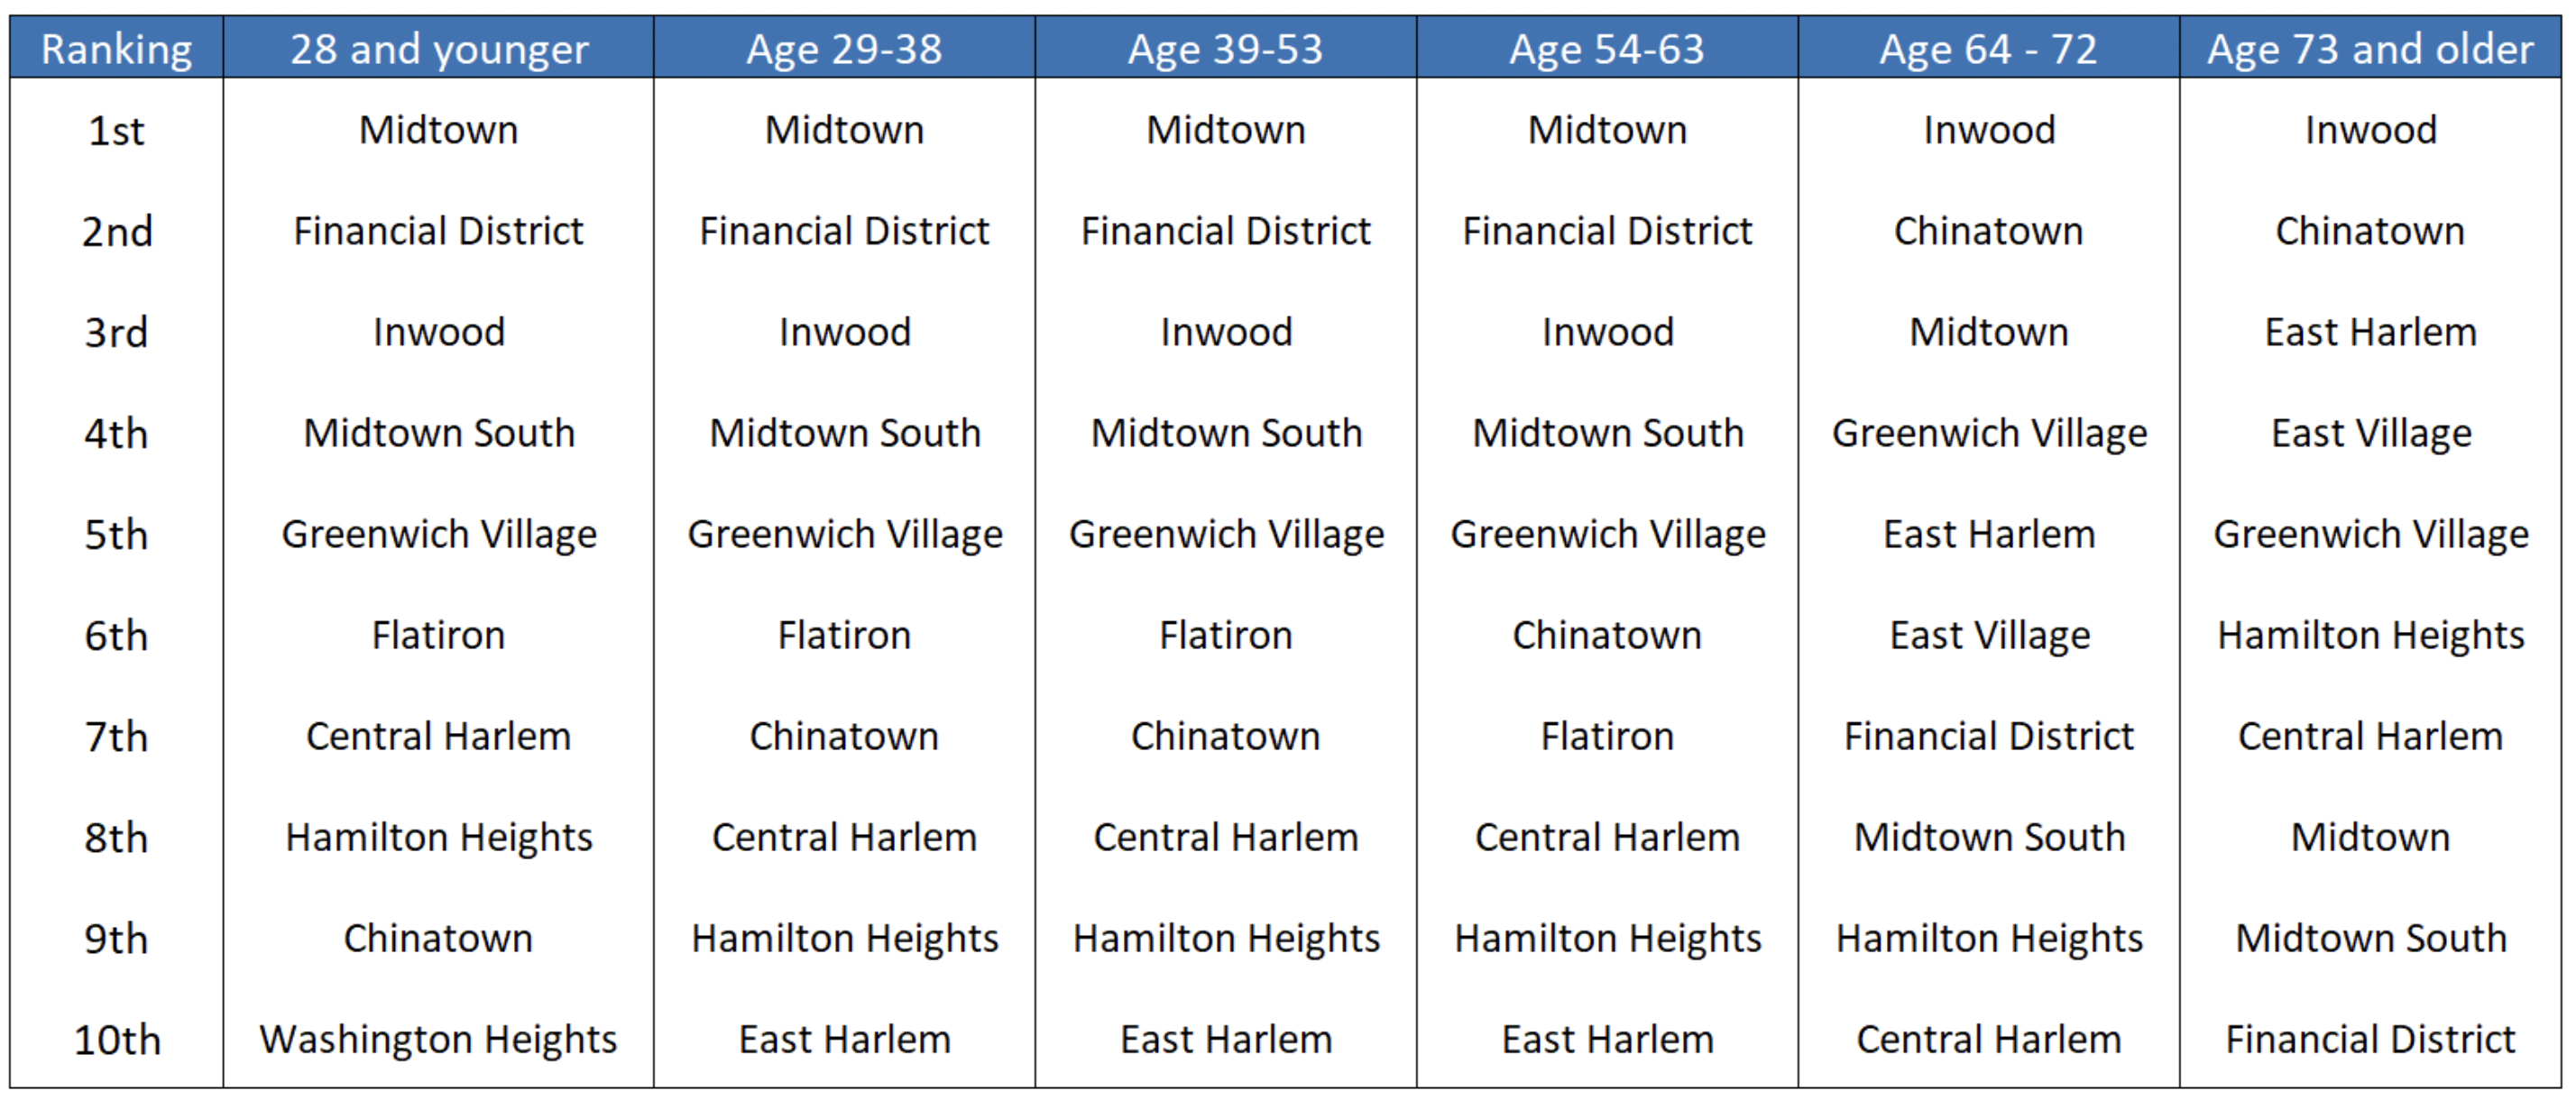
\includegraphics[scale=0.20]{final_results.png}
\end{figure}

Finally, we develop a map that illustrates the livability of each neighborhood. In addition, we design a recommendation system that allows users to input their age as shown in our video presentation. The system then generates personalized results, such as the example provided below, which displays the livability scores for different age groups. Specifically, it presents the livability score for a 25-year-old individual and a 30-year-old individual.

\begin{figure}[h]
\centering
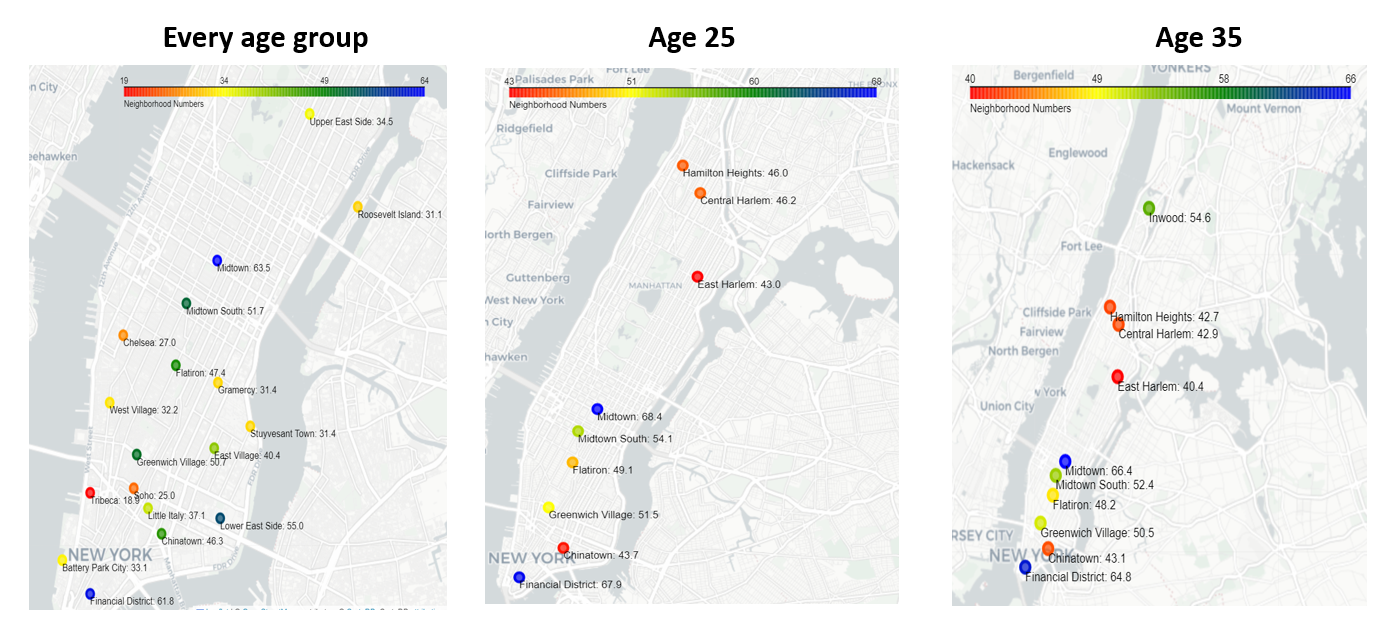
\includegraphics[scale=0.60]{map_score_reccom.png}
\end{figure}


\section{Conclusion}
In conclusion, there are many factors that contribute to a neighborhood's overall livability.  Overall sentiment and vibe of a neighborhood is a strong predictor of a neighborhood's livability and we were able to assess the sentiment of a neighborhood using Twitter data.  Affordability is another important factor of livability, and using rental data from Streeteasy, we identified the most and least affordable neighborhoods.  Easy access to restaurants and grocery stores plays another important role in a neighborhood; people like to have many options, and we noticed this preference is very strong amongst younger people.  More livable neighborhoods also have greater access to public transportation.  We calculated a neighborhood's convenience to public transportation using MTA's subway data and noticed a strong correlation between a high convenience score and the highest ranked neighborhoods.  We learned that there are many factors that can affect a neighborhood's livability and different age groups weigh these factors differently when choosing a neighborhood to live in.

\section{Contributions}
\begin{itemize}
\item Zain: Business understanding, data extraction \& cleaning/ exploratory data analysis (Doordash, Recognized Grocery Stores), mid-check point report, final project video and report
\item Hatsuo: Business understanding, prior work/ demographic research, score calculation logic, mid-check point report, slide deck, final project video and report
\item Ayush: Business understanding, data extraction \& cleaning/ exploratory data analysis (Yelp Dataset, Fusion Api), Combined Score Logic, mid-check point report, final project video and report
\item Matt: Business understanding, data extraction \& cleaning/ exploratory data analysis (Streeteasy, MTA), mid-check point report, final presentation/ recording
\item Steven: Business understanding, data extraction \& cleaning/ exploratory data analysis (Twitter), result visualization, recommendation system, mid-check point report, final project video and report
\end{itemize}

\section*{References}

[1] https://en.wikipedia.org/wiki/List\_of\_Manhattan\_neighborhoods \\

[2] AARP Livability Index: Great Neighborhoods for All Ages \ Public Policy Institute \ <https://www.aarp.org/ppi/issues/livable-communities/info-2015/livability-index.html> \ accessed 27/4/2022 \\

[3] Twitter Develop API manual \ <https://developer.twitter.com/en/docs/tutorials/filtering-tweets-by-location#introduction> \ accessed 27/4/2022 \\

[4] Sentiment Analysis using TextBlob \ Parthvi Shah \ <https://pypi.org/project/textblob/> \ accessed 27/4/2022 \\

[5] https://docs.developer.yelp.com/docs/fusion\-intro  

[6] 2019 Home Buyers and Sellers Generational Trends Report, Slide 36, https://www.nar.realtor/sites/default/files/documents/2019-home-buyers-and-sellers-generational-trends-report-08-16-2019.pdf \\

\end{document}